%%% ======= Beamer ======
\documentclass[usenames,dvipsnames,t]{beamer}
% \documentclass[usenames,dvipsnames, handout]{beamer}
\beamertemplatenavigationsymbolsempty % remove toolbar at the bottom of slides
\usepackage{appendixnumberbeamer} % for appendix
\usetheme{Madrid}
\usecolortheme{default}
\useinnertheme{circles}

\setbeamercolor{author in head/foot}{bg=blue!10, fg=blue}
\setbeamercolor{title in head/foot}{bg=blue!10, fg=blue}
\setbeamercolor{date in head/foot}{bg=blue!10, fg=blue}

\makeatletter
\setbeamertemplate{footline}{
  \leavevmode%
  \hbox{%
  \begin{beamercolorbox}[wd=.333333\paperwidth,ht=2.25ex,dp=1ex,center]{author in head/foot}%
    \usebeamerfont{author in head/foot}\insertshortauthor\expandafter\ifblank\expandafter{\beamer@shortinstitute}{}{~~(\insertshortinstitute)}
  \end{beamercolorbox}%
  \begin{beamercolorbox}[wd=.333333\paperwidth,ht=2.25ex,dp=1ex,center]{title in head/foot}%
    \usebeamerfont{title in head/foot}\insertshorttitle
  \end{beamercolorbox}%
  \begin{beamercolorbox}[wd=.333333\paperwidth,ht=2.25ex,dp=1ex,right]{date in head/foot}%
    \usebeamerfont{date in head/foot}\insertshortdate{}\hspace*{2em}
    \insertframenumber{}%
%     / \inserttotalframenumber
    \hspace*{2ex} 
  \end{beamercolorbox}}%
  \vskip0pt%
}
\makeatother

\colorlet{beamer@blendedblue}{blue!70} % change color theme


% For appendix
\newcommand{\backupbegin}{
   \newcounter{framenumberappendix}
   \setcounter{framenumberappendix}{\value{framenumber}}
}
\newcommand{\backupend}{
   \addtocounter{framenumberappendix}{-\value{framenumber}}
   \addtocounter{framenumber}{\value{framenumberappendix}} 
}

\setbeamertemplate{bibliography item}{\insertbiblabel} % improved references



% Other preamble stuff:
\usepackage{preamble}
\usepackage{fontawesome}

% Define commands for social media icons with links
\newcommand{\twitter}{\href{https://twitter.com/ThibeauWouters}{\textcolor{gray}{\faTwitter}}}
\newcommand{\linkedin}{\href{https://www.linkedin.com/in/ThibeauWouters}{\textcolor{gray}{\faLinkedin}}}
\newcommand{\github}{\href{https://github.com/ThibeauWouters}{\textcolor{gray}{\faGithub}}}



%%% Uncomment for another color palette
% \definecolor{Logo1}{rgb}{0.0, 0, 0.7}
% \definecolor{Logo2}{rgb}{2.55, 2.55, 2.55}

% \setbeamercolor*{palette primary}{bg=Logo1, fg=white}
% \setbeamercolor*{palette secondary}{bg=Logo2, fg=white}
% \setbeamercolor*{palette tertiary}{bg=white, fg=Logo1}
% \setbeamercolor*{palette quaternary}{bg=white,fg=white}
% \setbeamercolor{structure}{fg=Logo1} % itemize, enumerate, etc
% \setbeamercolor{section in toc}{fg=Logo1} % TOC sections

% For figures
\usepackage{import}
\usepackage{xifthen}
\usepackage{pdfpages}
\usepackage{transparent}
\usepackage{mdframed}

% --- Inkscape figures:
\newcommand{\incfig}[2][0.75\textwidth]{%
    \def\svgwidth{\columnwidth}
    \resizebox{#1}{!}{\import{Inkscape figs/}{#2.pdf_tex}}
}

% --- Height of frame
\newlength{\myheight}
\setlength{\myheight}{7cm}


%------------------------------------------------------------
%This block of code defines the information to appear in the
%Title page
\title[ML4GW: \texttt{jax}] %optional
{Machine Learning for Gravitational Waves: \texttt{jax}}

\author{Thibeau Wouters \vspace{5mm} \newline \github \quad \linkedin \quad \twitter}

\date{December 15, 2023}




%End of title page configuration block
%------------------------------------------------------------



%------------------------------------------------------------
%The next block of commands puts the table of contents at the 
%beginning of each section and highlights the current section:

\AtBeginSection[]
{
  \begin{frame}[plain, noframenumbering]
    \frametitle{Table of Contents}
    \tableofcontents[currentsection]
  \end{frame}
}

\AtBeginSubsection[]
{
  \begin{frame}[plain, noframenumbering]
    \frametitle{Table of Contents}
    \tableofcontents[currentsection]
  \end{frame}
}


%------------------------------------------------------------


\begin{document}

{

% \usebackgroundtemplate{\transparent{0.15}{
\includegraphics[width=\paperwidth,height=\paperheight]{Figures/ML4GWNL.png}}}

\begin{frame}[plain]
\titlepage

\vspace{-5mm}

\begin{figure}
\centering

\includegraphics[width=0.25\textwidth]{Figures/utrecht-university.png}
\end{figure}

\end{frame}
}

% %The next statement creates the title page.
% \frame[plain]{\titlepage



% }


%---------------------------------------------------------
%This block of code is for the table of contents after
%the title page
\begin{frame}[plain, noframenumbering]
\frametitle{Table of Contents}
\tableofcontents
\end{frame}
%---------------------------------------------------------


\section{Introduction}

\begin{frame}{Parameter estimation}

\def\x{3mm}
\def\y{2mm}

\begin{itemize}
    \item Parameter estimation (PE): get \red{posterior} of EM/GW parameters $\theta$ % from data $d$
    \begin{equation*}
        \red{p(\theta | d)} = \frac{p(d | \theta) p(\theta)}{p(d)}
    \end{equation*}

    \vspace{\y}

    \item Sampling via Markov Chain Monte Carlo (MCMC)~\cite{brooks2011handbook}
    
    % \vspace{\y}
    
    % \item Success
\end{itemize}

\vspace{\x}


\begin{tcolorbox}[colback=blue!10, boxrule=0pt]
  \textbf{Goal}: Improve algorithms with a \texttt{jax} implementation
\end{tcolorbox}


\centering
\incfig[0.9\textwidth]{MCMC_illustration}

\end{frame}

  
  \begin{frame}{Why \texttt{jax}?}
  
    \def\x{4mm}
  
    \begin{tcolorbox}[colback=blue!10, boxrule=0pt]
      What are the benefits of \texttt{jax} for MCMC?
    \end{tcolorbox}
  
  % \vspace{3mm}
  
  \begin{columns}
    \column{0.75\textwidth}
    \begin{enumerate}
      \item Automatic differentiation (AD)
      
      \vspace{\x}
  
      \item Just-in-time (JIT) compilation
      
      \vspace{\x}
      
      \item GPU acceleration
      
      \vspace{\x}
      
      \item Parallelization
      
      \vspace{\x}
      
      \item Shown to speed up PE for GWs~\cite{wong2023fast}, cosmology~\cite{piras2023cosmopower},...
      
      % \vspace{\x}
      
      % \item Interoperability with \texttt{numpy}
    \end{enumerate}
    \column{0.20\textwidth}
    \begin{figure}
      % \centering
      
\includegraphics[width=\textwidth]{Figures/jax.png}
    \end{figure}
  \end{columns}
    
  \end{frame}

\begin{frame}{What is my experience with \texttt{jax}?}

  \def\x{5mm}

  \begin{enumerate}
    \item TaylorF2, NRTidalv2 GW in \texttt{ripple}~\cite{edwards2023ripple}
    
    \vspace{\x}

    \item Worked with \texttt{flowMC}~\cite{gabrie2021efficient, wong2022flowmc}, a gradient-based, normalizing flow-enhanced MCMC sampler
    
    \vspace{\x}

    \item Worked on \texttt{jim}~\cite{wong2023fast}, a PE pipeline for GWs (see appendix of this presentation for more information)
    
    \vspace{\x}

    \item Implemented kilonova surrogate models in \texttt{flax}~\cite{flax2020github} for \texttt{NMMA}~\cite{pang2022nmma}
  \end{enumerate}

  \vspace{5mm}

  \begin{tcolorbox}[colback=blue!10, boxrule=0pt]
    What are some take-aways for getting started with \texttt{jax}?
  \end{tcolorbox}
  
\end{frame}

\section{Some \texttt{jax} take-aways}

\begin{frame}{\#1 -- Don't be scared, just try it out!}

  \def\x{6mm}

  \begin{itemize}
    \item \texttt{jax} is easy to get started with: \texttt{numpy} $\rightarrow$ \texttt{jax.numpy} works well!
    
    \vspace{\x}

    \item What about large projects?
    
    \begin{itemize}
      \vspace{\x}

      \item Make sure to read the \href{https://jax.readthedocs.io/en/latest/notebooks/Common_Gotchas_in_JAX.html}{``sharp bits''} \
      
      \vspace{\x}

      \item Check out other repositories for inspiration (\href{https://github.com/n2cholas/awesome-jax}{list of repos})

      \vspace{\x}
      
      \item Read/watch some tutorials, such as \href{https://github.com/gordicaleksa/get-started-with-JAX}{this one}
      
      \vspace{\x}
      
      \item Large project? \textit{Start from scratch!}
      
      % \vspace{\x}

      % \item Arrays are immutable
      
      % \vspace{\x}

      % \item Functions must be pure for jitting
      
      % \vspace{\x}

      % \item Random numbers are a bit annoying
    \end{itemize}
  \end{itemize}

  \vspace{3mm}

  \href{https://github.com/ThibeauWouters/jax-getting-started/blob/main/jax-getting-started.ipynb}{Small demo} about first caveats
  
\end{frame}

\begin{frame}{\#2 -- Functions must be pure: conditionals}

  Example: \texttt{lalsuite} vs \texttt{jax} for NRTidalv2

  \vspace{-2mm}

  \begin{columns}

    \column{0.9\textwidth}
    \begin{figure}[H]
      \centering
      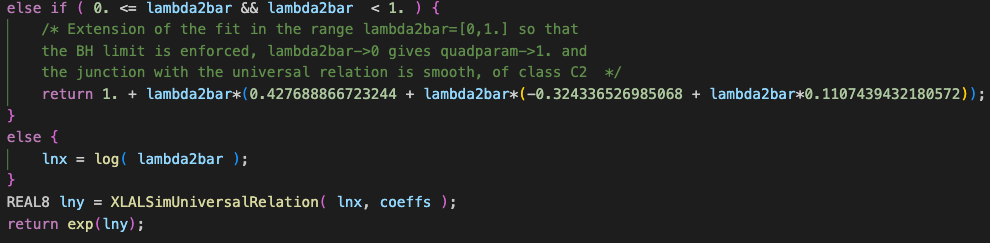
\includegraphics[width=0.8\textwidth]{Figures/lalsuite_code.png}
    \end{figure}
  
    \begin{figure}[H]
      \centering
      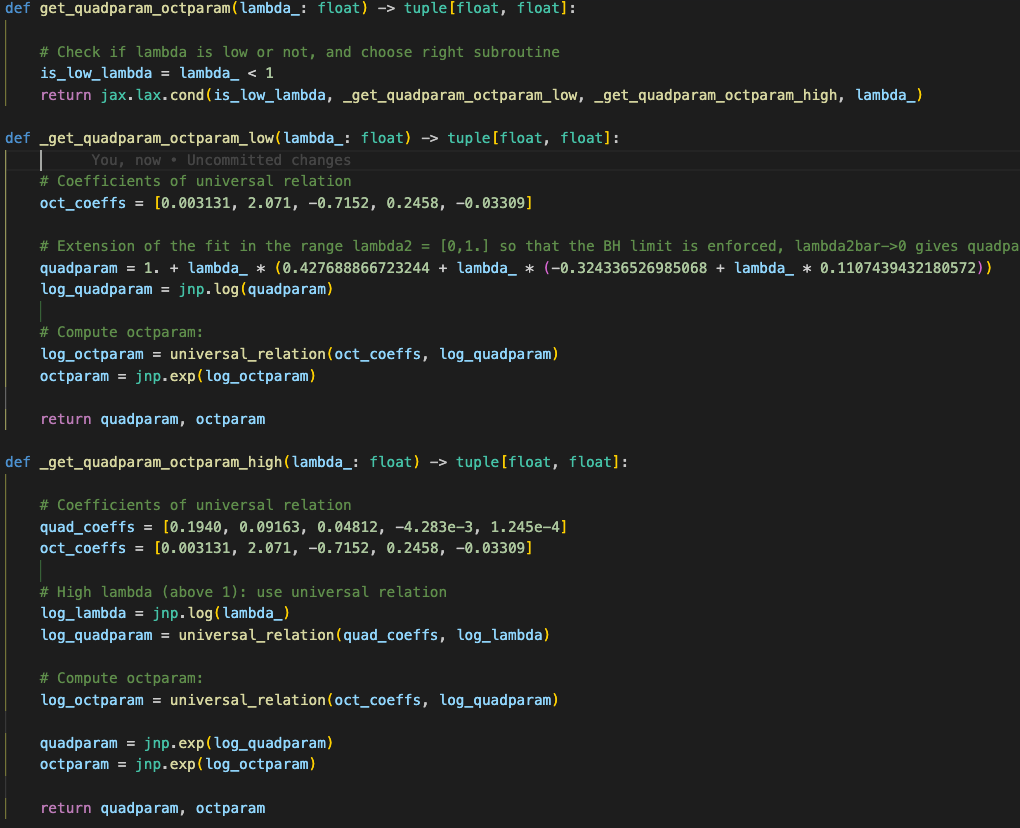
\includegraphics[width=0.8\textwidth]{Figures/ripple_code.png}
    \end{figure}
  
    \column{0.15\textwidth}

    \vspace{1cm}

    \texttt{lalsuite} 

    \vspace{3cm}

    \texttt{jax} 

    (\href{https://github.com/ThibeauWouters/ripple/blob/main/src/ripple/waveforms/utils_tidal.py}{code})
  
  \end{columns}

\end{frame}


\begin{frame}{\#3 Neural networks}


  \def\x{3mm}

  Neural networks in \texttt{flax}:

  \vspace{\x}

  \begin{itemize}
    \item Most similar to \texttt{PyTorch}, more work than \texttt{tensorflow}
    
    \vspace{\x}

    \item \texttt{flax} has a different ``mindset'' 
    
    \vspace{\x}
    
    \item Check out my very basic \href{https://github.com/ThibeauWouters/jax-getting-started/blob/0e4b45133794f86028423b6b4814471e068ef2d3/flax/utils_flax.py\#L183}{flax code}
  \end{itemize}
  
  \centering
  \incfig[\textwidth]{drawing}
  
\end{frame}

\section{Conclusion}

\begin{frame}{Conclusion}

  \def\x{7mm}

  \begin{itemize}
    \item \texttt{jax} is a great tool to speed up code
    
    \vspace{\x}

    \item \texttt{jax} is easy, but watch out for the ``sharp bits''
    
    \vspace{\x}

    \item \texttt{flax} implements neural networks with \texttt{jax}
    
    \vspace{\x}

    \item Interested? Let's connect and learn together!
  \end{itemize}

  \vspace{5mm}
  
  \begin{tcolorbox}[colback=blue!10, boxrule=0pt]
    Thanks for listening! Questions?
  \end{tcolorbox}

\end{frame}


% ======== APPENDIX  ==========

% \appendix

\section{Appendix: GW parameter estimation with \texttt{jax}}
\begin{frame}{Overview}

    % % \def\x{2mm}

% We extend \texttt{jim} \cite{wong2023fast}, based on \texttt{jax} \cite{jax2018github}, with building blocks:
% \vspace{2mm}
% \begin{enumerate}
%   % \item 
  
%   % \vspace{\x}

%   \item Normalizing flow-enhanced, gradient-based MCMC (\texttt{flowMC}, \cite{gabrie2021efficient, wong2022flowmc})
  
%   \vspace{\x}

%   \item Automatically-differentiable (AD) GW (\texttt{ripple} \cite{edwards2023ripple})
  
%   \vspace{\x}

%   \item \gray{Relative binning likelihood \cite{zackay2018relative}}
% \end{enumerate}

% \vspace{-3mm}

% \incfig[\textwidth]{jim_flowMC_ripple}
    \def\x{2mm}
  
  We extend \texttt{jim} \cite{wong2023fast}, based on \texttt{jax} \cite{jax2018github}, with building blocks:
  \vspace{2mm}
  \begin{enumerate}
    % \item 
    
    % \vspace{\x}
  
    \item Normalizing flow-enhanced, gradient-based MCMC (\texttt{flowMC}~\cite{gabrie2021efficient, wong2022flowmc})
    
    \vspace{\x}
  
    \item Automatically-differentiable (AD) GW (\texttt{ripple}~\cite{edwards2023ripple})
    
    \vspace{\x}
  
    \item \gray{Relative binning likelihood~\cite{zackay2018relative}}
  \end{enumerate}
  
  \vspace{-3mm}
  
  \incfig[\textwidth]{jim_flowMC_ripple}
    
  \end{frame}
  
  % % \section{Why \texttt{jax}?}
  
  % \begin{frame}{Why \texttt{jax}?}
  
  %   \def\x{4mm}
  
  %   \begin{tcolorbox}[colback=blue!10, boxrule=0pt]
  %     What are the benefits of \texttt{jax} for MCMC?
  %   \end{tcolorbox}
  
  % \vspace{3mm}
  
  % \begin{columns}
  %   \column{0.75\textwidth}
  %   \begin{enumerate}
  %     \item Automatic differentiation (AD)
      
  %     \vspace{\x}
  
  %     \item Just-in-time (JIT) compilation
      
  %     \vspace{\x}
      
  %     \item GPU acceleration
      
  %     \vspace{\x}
      
  %     \item Parallelization
      
  %     % \vspace{\x}
      
  %     % \item Vectorization
      
  %     % \vspace{\x}
      
  %     % \item Interoperability with \texttt{numpy}
  %   \end{enumerate}
  %   \column{0.20\textwidth}
  %   \begin{figure}
  %     % \centering
  %     
\includegraphics[width=\textwidth]{Figures/jax.png}
  %   \end{figure}
  % \end{columns}
    
  % \end{frame}
  
  % \section{\texttt{flowMC}}
  
  \begin{frame}{\texttt{flowMC} -- local sampling}
  
  \begin{enumerate}
    \item \textbf{Local sampling}: MALA (Metropolis-adjusted Langevin algorithm)
    
    \vspace{3mm}
    
    \begin{itemize}
      \item Proposal \red{$y$}: Langevin diffusion
      \begin{equation*}
        \red{y} = x + \frac{\epsilon^2}{2} \nabla \log p(x) + \epsilon \xi
      \end{equation*}
  
      \item Metropolis-Hastings acceptance step
      
      \vspace{3mm}

      \item Motivates the need for automatic differentiation
    \end{itemize}
    
  \end{enumerate}
  
  \incfig[\textwidth]{MALA}
  
  \end{frame}
  
  
  
  \begin{frame}{\texttt{flowMC} -- normalizing flows}
  
  \def\x{3mm}
  \def\y{5mm}
  
  Normalizing flows (NF):
  
  \vspace{\x}
  
  \begin{itemize}
    \item \blue{Latent space}: easy to sample (e.g. Gaussian)
    
    \vspace{\x}
  
    \item \red{Data space}: distribution learned from samples
    
    \vspace{\x}
    
    \item Enable approximate sampling from complicated distributions
  \end{itemize}
  
  \vspace{\y}
    
  \incfig[\textwidth]{NF}
  
  \end{frame}
  
  
  \begin{frame}{\texttt{flowMC} -- global sampling}
  
    \def\x{3mm}
    \def\y{2mm}
  
    \begin{enumerate}
      \setcounter{enumi}{1}
      \item \textbf{Global sampling}
    \end{enumerate}
  
    \vspace{\x}
  
    \begin{itemize}
      \item Global proposal by sampling from NF
      
      \vspace{\y}
      
      \item Metropolis-Hastings acceptance step
    \end{itemize}
  
    \vspace{8mm}
    
    \incfig[\textwidth]{global_sampling}
  
  \end{frame}
  
  
  
  \begin{frame}{\texttt{flowMC} -- complete algorithm}
  
    \only<1>{\textbf{Training loop} \& Production loop}
    \only<2>{Training loop \& \textbf{Production loop}}
  
    \vspace{-5mm}  
    
    \only<1>{
      \incfig[\textwidth]{flowMC_loop}
    }
  
    \only<2>{
      \vspace{1cm}
      \incfig[\textwidth]{flowMC_loop_production}
    }
  
  \end{frame}
  
  
  % \section{Results}
  
  \begin{frame}{Results}
    \def\x{2mm}
    \def\y{-3mm}
  
  
    % Tidal waveform models in \texttt{ripple}:
    \begin{itemize}
      \item TaylorF2 in \texttt{ripple}
      
      \vspace{\x}
  
      \item IMRPhenomD\_NRTidalv2 in \texttt{ripple} (ongoing)
      
      \vspace{\x}
      
      \item Reproduced PE for GW170817 \& GW190425 with TaylorF2
      
      \vspace{\x}
  
      \item $\sim 30$ mins training, $\sim 1$ min sampling
    \end{itemize}
  
    \vspace{\y}
  
    % \incfig[\textwidth]{jim_flowMC_ripple}
    \vspace{8mm}
    \begin{figure}[H]
      \centering
      % 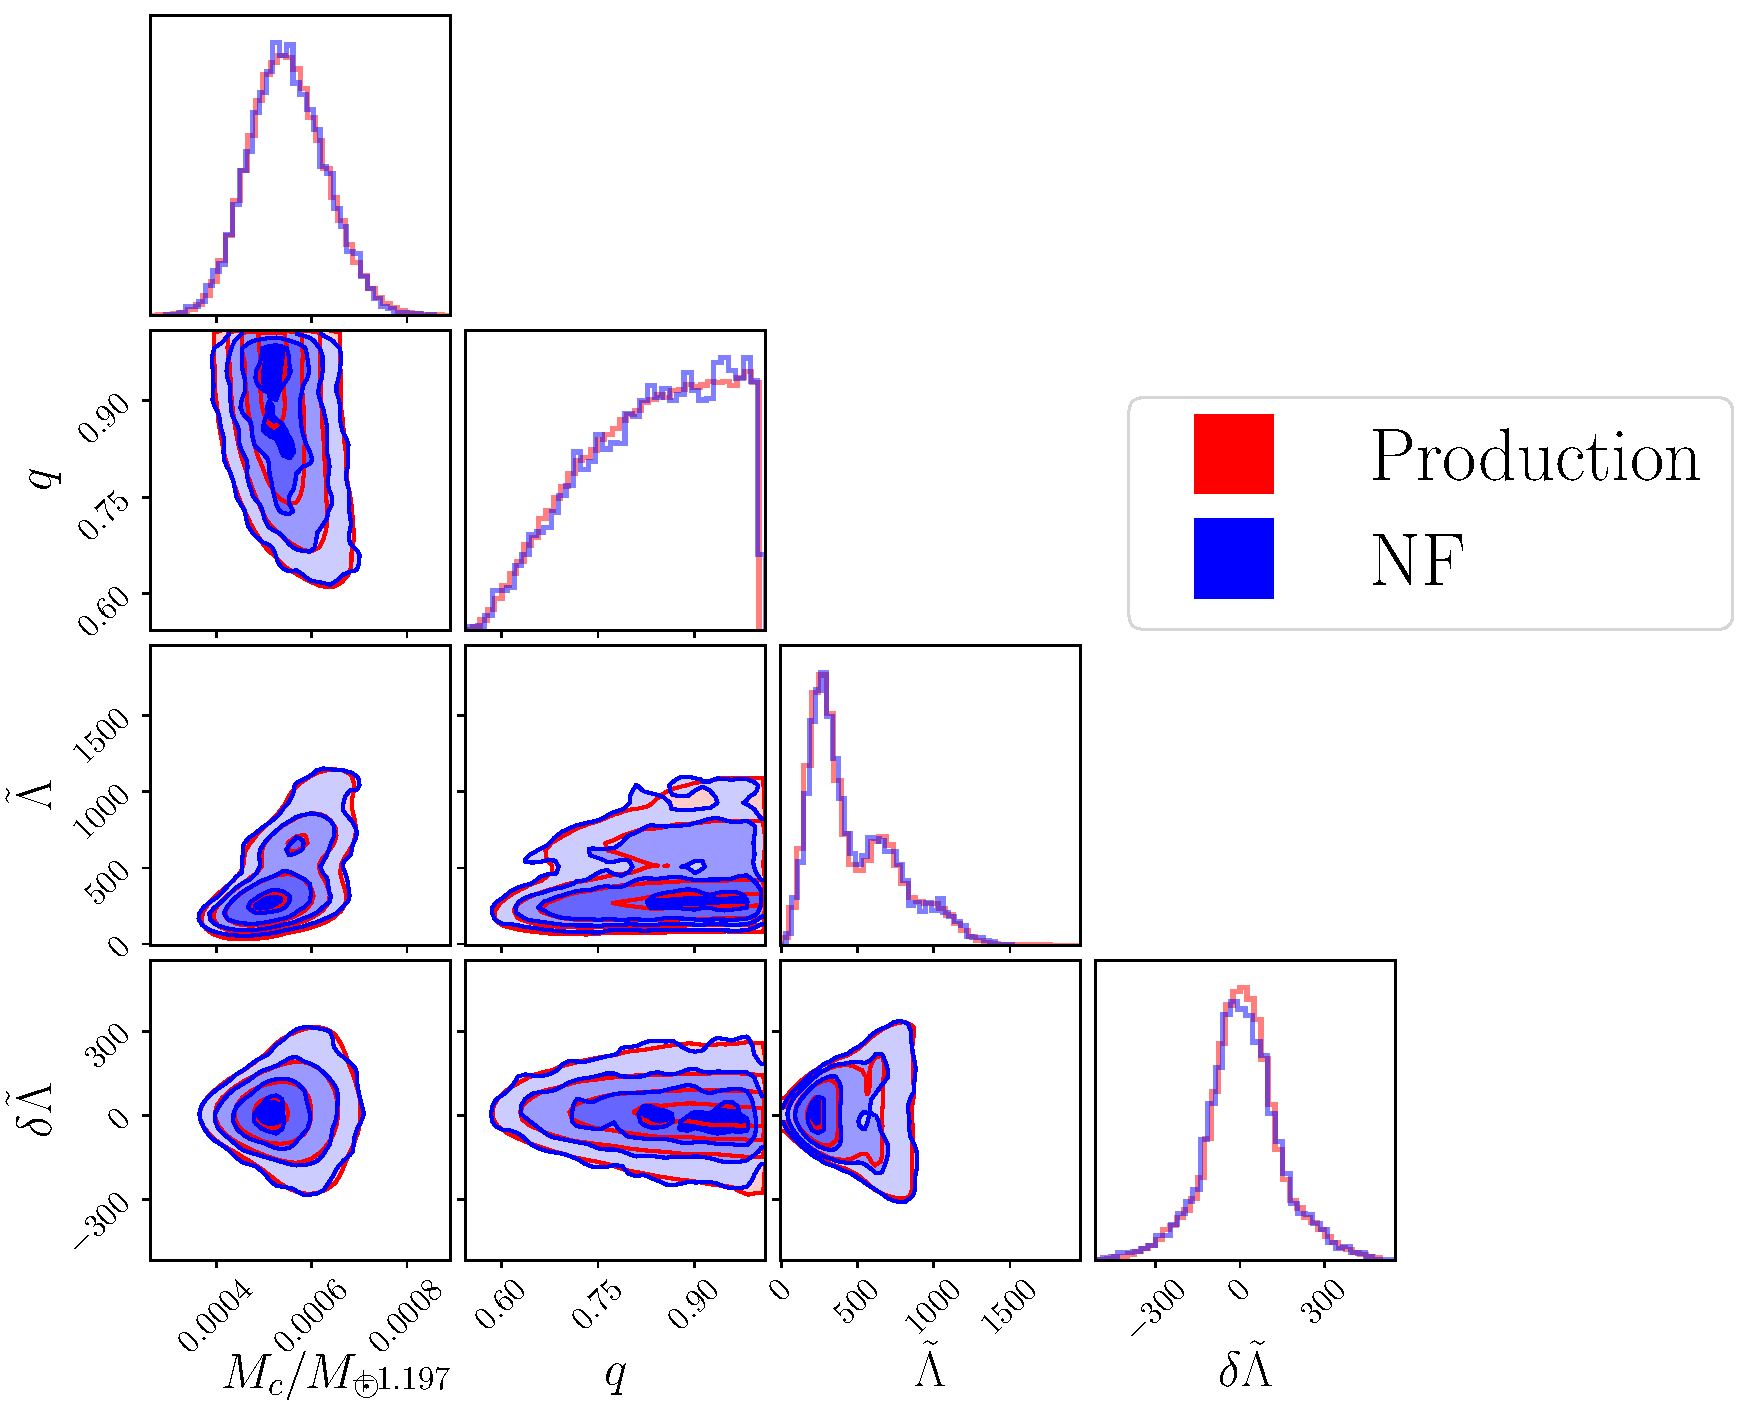
\includegraphics[scale=0.2]{Figures/presentation_GW170817_production_vs_NF_masses.pdf}
      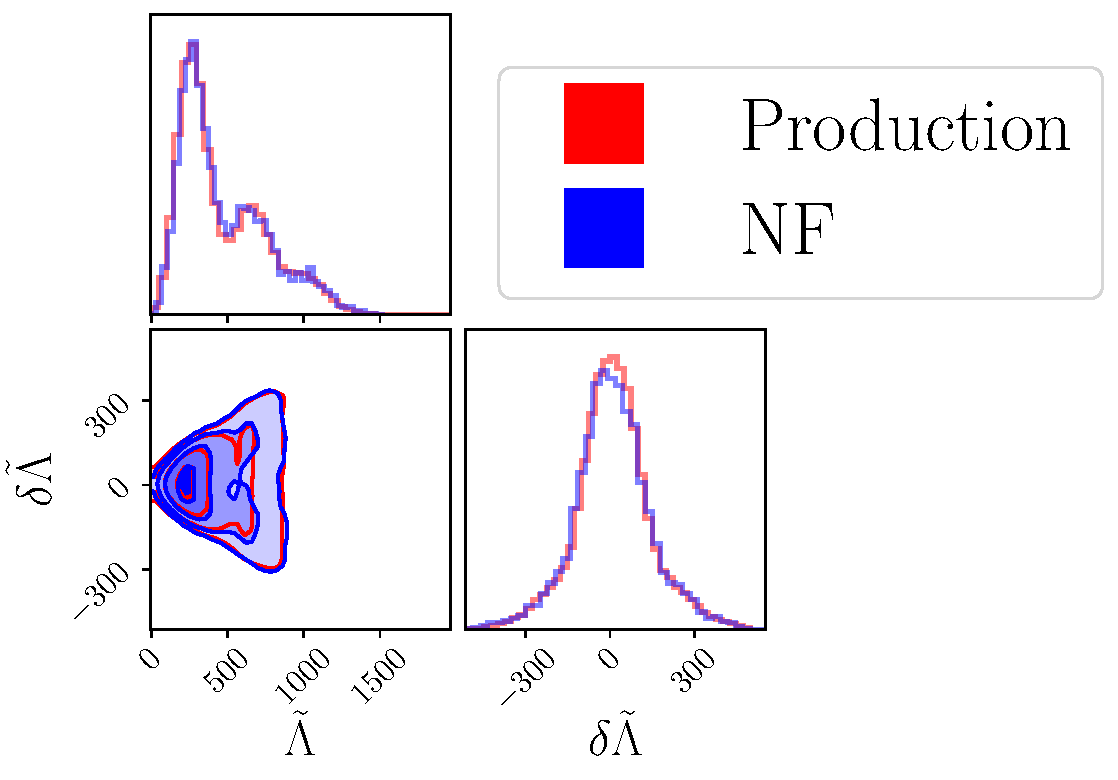
\includegraphics[width = 0.55\textwidth]{Figures/presentation_GW170817_production_vs_NF.pdf}
    \end{figure}
  \end{frame}
  
  
  % \section{Future work \& conclusion}
  
  % \begin{frame}{Future work}
  
  %   \def\x{6mm}
  
  %   \vspace{4mm}
  
  %   \begin{itemize}
  %     \item Finish IMRPhenomD\_NRTidalv2 in \texttt{ripple}
      
  %     \vspace{\x}
      
  %     \item Injection studies and pp-plot
      
  %     \vspace{\x}
  
  %     \item Update NF settings, boost efficiency
      
  %     \vspace{\x}
      
  %     \item Investigate synergy with simulation-based inference (\red{let's talk!})
      
  %     % \vspace{\x}
      
  %     % \item Investigate possibility of pretraining
  %   \end{itemize}
  
  % \end{frame}
  
  % \begin{frame}{Conclusion}
  
  %   \def\x{2mm}
  
  %   \begin{itemize}
  %     \item \texttt{flowMC}: NF-enhanced, gradient-based MCMC
      
  %     \vspace{\x}
      
  %     \item \texttt{ripple}: automatically differentiable GW
      
  %     \vspace{\x}
      
  %     \item $\texttt{jim} = \texttt{jax} + \texttt{flowMC} + \texttt{ripple}$
      
  %     % \vspace{\x}
      
  %     % \item \texttt{jim} is a promising tool for fast and accurate parameter estimation
      
  %     \vspace{\x}
  
  %     \item \texttt{jim} can do PE of BNS in $\sim 1$ min sampling/$\sim 30$ min wall time
      
  %     \vspace{\x}
      
  %     % \item \texttt{jim} can enhance and benefit from simulation-based inference
      
  %   \end{itemize}
  
  %   \vspace{-5mm}
  
  %   \incfig[\textwidth]{jim_flowMC_ripple}
      
  % \end{frame}
  
  % \begin{frame}[plain, noframenumbering]{References}
  
  % \printbibliography
      
  % \end{frame}

\end{document}

